\documentclass[crop=true,tikz,border=1pt,varwidth=8in]{standalone}

\usepackage{amsmath}
%\makeatletter
%%%%%%%%%%%%%%%%%
\PassOptionsToPackage{force}{filehook}
\usepackage{tikz}
\usetikzlibrary{shapes,arrows}
\usetikzlibrary{positioning}
\tikzstyle{cloud} = [draw, ellipse,fill=red!20, node distance=0.87cm,
minimum height=2em]
\tikzstyle{line} = [draw, -latex']
\usetikzlibrary{shapes.symbols,shapes.callouts,patterns}
\usetikzlibrary{calc,fit}
\usetikzlibrary{backgrounds}


\begin{document}
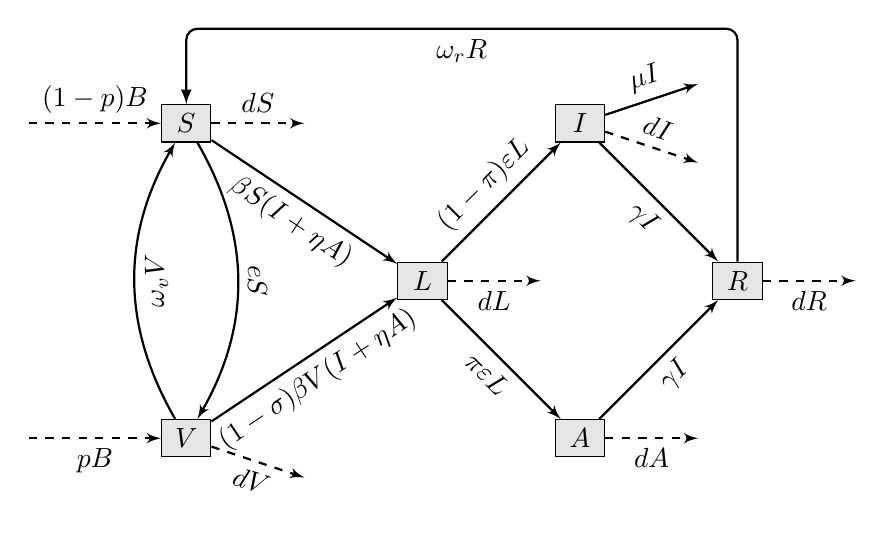
\begin{tikzpicture}[scale=1, every node/.style={transform shape},
	auto, %node distance = 2cm, auto,
	box/.style={minimum width={width("N-1")+2pt},
		draw, rectangle,fill=gray!20}]
	%% States
	\node [box] at (0,2) (S) {$S$};
	\node [box] at (0,-2) (V) {$V$};
	\node [box] at (3,0) (L) {$L$};
	\node [box] at (5,2) (I) {$I$};
	\node [box] at (5,-2) (A) {$A$};
	\node [box] at (7,0) (R) {$R$};
	%% Flows
	\path [line, thick, dashed] (-2,2) to node [midway, above] (TextNode) {$(1-p)B$} (S);
	\path [line, thick, dashed] (-2,-2) to node [midway, below] (TextNode) {$pB$} (V);
	\path [line, thick] (S) to node [midway, below, sloped] (TextNode) {$\beta S(I+\eta A)$} (L);
	\path [line, thick, bend left] (S) to node [midway, above, sloped] (TextNode) {$eS$} (V);
	\path [line, thick, bend left] (V) to node [sloped, midway, below] (TextNode) {$\omega_v V$} (S);
	\path [line, thick] (V) to node [midway, below, sloped] (TextNode) {$(1-\sigma)\beta V(I+\eta A)$} (L);
	\path [line, thick] (L) to node [sloped, midway, above] (TextNode) {$(1-\pi)\varepsilon L$} (I);
	\path [line, thick] (L) to node [sloped, midway, below] (TextNode) {$\pi\varepsilon L$} (A);
	\path [line, thick] (I) to node [sloped, midway, below] (TextNode) {$\gamma I$} (R);
    \path [line, thick] (A) to node [sloped, midway, below] (TextNode) {$\gamma I$} (R);
	\draw [>=latex,->, thick, rounded corners] (R) -- +(0,3.2) -- ++(-7,3.2) node[sloped, midway, below] {$\omega_r R$} -- (S);
    \path [line, thick, dashed] (S) to node [sloped, midway, above] (TextNode) {$dS$} ++(1.5,0);
    \path [line, thick, dashed] (V) to node [sloped, midway, below] (TextNode) {$dV$} ++(1.5,-0.5);
    \path [line, thick, dashed] (L) to node [sloped, midway, below] (TextNode) {$dL$} ++(1.5,0);
    \path [line, thick, dashed] (I) to node [sloped, midway, above] (TextNode) {$dI$} ++(1.5,-0.5);
    \path [line, thick] (I) to node [sloped, midway, above] (TextNode) {$\mu I$} ++(1.5,0.5);
    \path [line, thick, dashed] (A) to node [sloped, midway, below] (TextNode) {$dA$} ++(1.5,0);
    \path [line, thick, dashed] (R) to node [sloped, midway, below] (TextNode) {$dR$} ++(1.5,0);
\end{tikzpicture}
\end{document}